\batchmode
\documentclass{book}
\RequirePackage{ifthen}




\usepackage{tesis_estilo}


\usepackage{graphicx}

%
\providecommand{\titleGM} {\begingroup% Create the command for including the title page in the document
	\titlepage		% saco el número de página de la carátula
	\hbox{ % Horizontal box
		\hspace*{0.2\textwidth} % Whitespace to the left of the title page
		\rule{1pt}{\textheight} % Vertical line
		\hspace*{0.05\textwidth} % Whitespace between the vertical line and title page text
		\parbox[b]{0.75\textwidth}{ % Paragraph box which restricts text to less than the width of the page
			

{\noindent\Huge\bfseries LTITOOL \\}\\[2\baselineskip] % Title
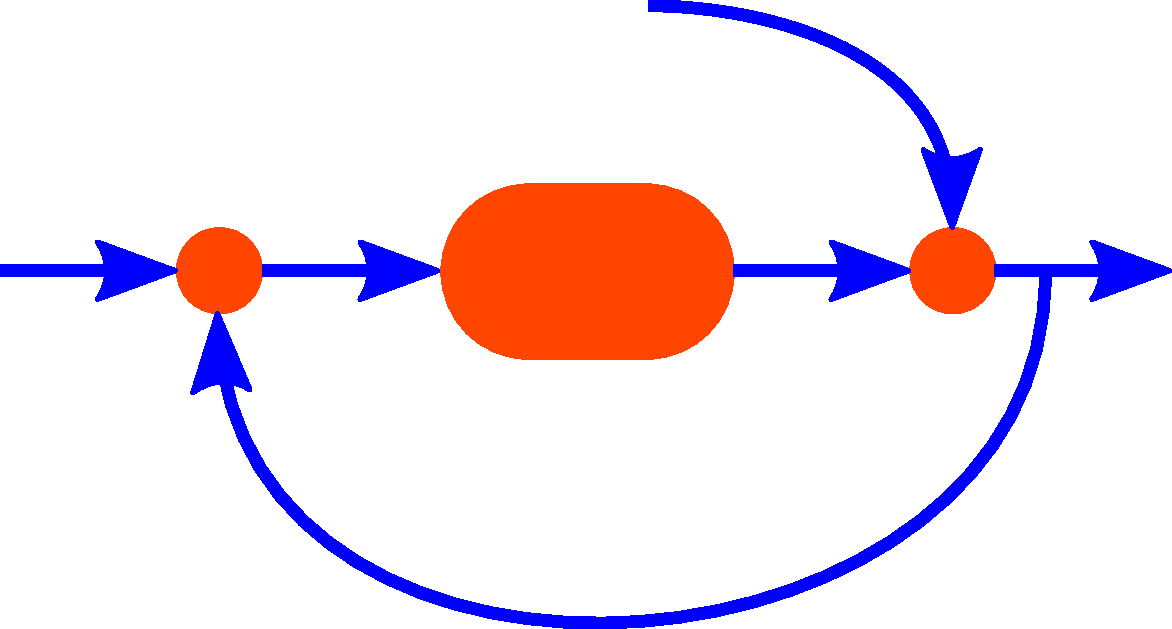
\includegraphics[scale=0.3]{./figuras/logos/logo_ltitool.png}


{\large \textit{\\LTI Control System Toolbox}}\\[4\baselineskip] % Tagline or further description
			{\large \textsc{ Eduardo J. Adam }} % Author name
			

\vspace{0.5\textheight} % Whitespace between the title block and the publisher
			{\noindent \textsc{A\~{n}o:} \Year }\\[\baselineskip] % Publisher and logo
	}


}
	%


\textbf{Developers and Collaborators of this edition:}


\vspace{0.4cm}
\textsc{Eduardo J. Adam}, (\url{eadam.fiq@gmail.com})


Faculta de Ingeniería Química - Universidad Nacional del Litoral,


Santa Fe, Santa Fe, Argentina.


\vspace{2cm}
\textbf{Special thanks:}


\vspace{0.4cm}
Special thanks to Ernesto S. Burgos for the development of the GUI-Editor and for


for his selfless collaboration, which would otherwise it has made it impossible 


to achieve the GUIs here presented.


\vspace{0.2cm}
\textsc{Ernesto S. Burgos}, (\url{e.sergio.burgos@gmail.com})


Universidad Tecnoloógica Nacional - Facultad Regional Paraná,


Paraná, Entre Ríos, Argentina
.	\endgroup}




\usepackage{xcolor}

\usepackage[latin1]{inputenc}



\makeatletter
\AtBeginDocument{\makeatletter
\input /home/eadam/Dropbox/eadam/Desktop/escritorio/proyecto_sergio/ltitoolEnDesarrollo/version1.0.0/help/ltitool_manual/ltitool_manual.aux
\makeatother
}
\AtBeginDocument{\makeatletter
\input /home/eadam/Dropbox/eadam/Desktop/escritorio/proyecto_sergio/ltitoolEnDesarrollo/version1.0.0/help/ltitool_manual/chapter_intro.aux
\makeatother
}
\AtBeginDocument{\makeatletter
\input /home/eadam/Dropbox/eadam/Desktop/escritorio/proyecto_sergio/ltitoolEnDesarrollo/version1.0.0/help/ltitool_manual/chapter_install.aux
\makeatother
}
\AtBeginDocument{\makeatletter
\input /home/eadam/Dropbox/eadam/Desktop/escritorio/proyecto_sergio/ltitoolEnDesarrollo/version1.0.0/help/ltitool_manual/chapter_la.aux
\makeatother
}
\AtBeginDocument{\makeatletter
\input /home/eadam/Dropbox/eadam/Desktop/escritorio/proyecto_sergio/ltitoolEnDesarrollo/version1.0.0/help/ltitool_manual/chapter_lc.aux
\makeatother
}
\AtBeginDocument{\makeatletter
\input /home/eadam/Dropbox/eadam/Desktop/escritorio/proyecto_sergio/ltitoolEnDesarrollo/version1.0.0/help/ltitool_manual/chapter_eca.aux
\makeatother
}
\AtBeginDocument{\makeatletter
\input /home/eadam/Dropbox/eadam/Desktop/escritorio/proyecto_sergio/ltitoolEnDesarrollo/version1.0.0/help/ltitool_manual/chapter_additool.aux
\makeatother
}

\makeatletter
\count@=\the\catcode`\_ \catcode`\_=8 
\newenvironment{tex2html_wrap}{}{}%
\catcode`\<=12\catcode`\_=\count@
\newcommand{\providedcommand}[1]{\expandafter\providecommand\csname #1\endcsname}%
\newcommand{\renewedcommand}[1]{\expandafter\providecommand\csname #1\endcsname{}%
  \expandafter\renewcommand\csname #1\endcsname}%
\newcommand{\newedenvironment}[1]{\newenvironment{#1}{}{}\renewenvironment{#1}}%
\let\newedcommand\renewedcommand
\let\renewedenvironment\newedenvironment
\makeatother
\let\mathon=$
\let\mathoff=$
\ifx\AtBeginDocument\undefined \newcommand{\AtBeginDocument}[1]{}\fi
\newbox\sizebox
\setlength{\hoffset}{0pt}\setlength{\voffset}{0pt}
\addtolength{\textheight}{\footskip}\setlength{\footskip}{0pt}
\addtolength{\textheight}{\topmargin}\setlength{\topmargin}{0pt}
\addtolength{\textheight}{\headheight}\setlength{\headheight}{0pt}
\addtolength{\textheight}{\headsep}\setlength{\headsep}{0pt}
\setlength{\textwidth}{349pt}
\newwrite\lthtmlwrite
\makeatletter
\let\realnormalsize=\normalsize
\global\topskip=2sp
\def\preveqno{}\let\real@float=\@float \let\realend@float=\end@float
\def\@float{\let\@savefreelist\@freelist\real@float}
\def\liih@math{\ifmmode$\else\bad@math\fi}
\def\end@float{\realend@float\global\let\@freelist\@savefreelist}
\let\real@dbflt=\@dbflt \let\end@dblfloat=\end@float
\let\@largefloatcheck=\relax
\let\if@boxedmulticols=\iftrue
\def\@dbflt{\let\@savefreelist\@freelist\real@dbflt}
\def\adjustnormalsize{\def\normalsize{\mathsurround=0pt \realnormalsize
 \parindent=0pt\abovedisplayskip=0pt\belowdisplayskip=0pt}%
 \def\phantompar{\csname par\endcsname}\normalsize}%
\def\lthtmltypeout#1{{\let\protect\string \immediate\write\lthtmlwrite{#1}}}%
\newcommand\lthtmlhboxmathA{\adjustnormalsize\setbox\sizebox=\hbox\bgroup\kern.05em }%
\newcommand\lthtmlhboxmathB{\adjustnormalsize\setbox\sizebox=\hbox to\hsize\bgroup\hfill }%
\newcommand\lthtmlvboxmathA{\adjustnormalsize\setbox\sizebox=\vbox\bgroup %
 \let\ifinner=\iffalse \let\)\liih@math }%
\newcommand\lthtmlboxmathZ{\@next\next\@currlist{}{\def\next{\voidb@x}}%
 \expandafter\box\next\egroup}%
\newcommand\lthtmlmathtype[1]{\gdef\lthtmlmathenv{#1}}%
\newcommand\lthtmllogmath{\dimen0\ht\sizebox \advance\dimen0\dp\sizebox
  \ifdim\dimen0>.95\vsize
   \lthtmltypeout{%
*** image for \lthtmlmathenv\space is too tall at \the\dimen0, reducing to .95 vsize ***}%
   \ht\sizebox.95\vsize \dp\sizebox\z@ \fi
  \lthtmltypeout{l2hSize %
:\lthtmlmathenv:\the\ht\sizebox::\the\dp\sizebox::\the\wd\sizebox.\preveqno}}%
\newcommand\lthtmlfigureA[1]{\let\@savefreelist\@freelist
       \lthtmlmathtype{#1}\lthtmlvboxmathA}%
\newcommand\lthtmlpictureA{\bgroup\catcode`\_=8 \lthtmlpictureB}%
\newcommand\lthtmlpictureB[1]{\lthtmlmathtype{#1}\egroup
       \let\@savefreelist\@freelist \lthtmlhboxmathB}%
\newcommand\lthtmlpictureZ[1]{\hfill\lthtmlfigureZ}%
\newcommand\lthtmlfigureZ{\lthtmlboxmathZ\lthtmllogmath\copy\sizebox
       \global\let\@freelist\@savefreelist}%
\newcommand\lthtmldisplayA{\bgroup\catcode`\_=8 \lthtmldisplayAi}%
\newcommand\lthtmldisplayAi[1]{\lthtmlmathtype{#1}\egroup\lthtmlvboxmathA}%
\newcommand\lthtmldisplayB[1]{\edef\preveqno{(\theequation)}%
  \lthtmldisplayA{#1}\let\@eqnnum\relax}%
\newcommand\lthtmldisplayZ{\lthtmlboxmathZ\lthtmllogmath\lthtmlsetmath}%
\newcommand\lthtmlinlinemathA{\bgroup\catcode`\_=8 \lthtmlinlinemathB}
\newcommand\lthtmlinlinemathB[1]{\lthtmlmathtype{#1}\egroup\lthtmlhboxmathA
  \vrule height1.5ex width0pt }%
\newcommand\lthtmlinlineA{\bgroup\catcode`\_=8 \lthtmlinlineB}%
\newcommand\lthtmlinlineB[1]{\lthtmlmathtype{#1}\egroup\lthtmlhboxmathA}%
\newcommand\lthtmlinlineZ{\egroup\expandafter\ifdim\dp\sizebox>0pt %
  \expandafter\centerinlinemath\fi\lthtmllogmath\lthtmlsetinline}
\newcommand\lthtmlinlinemathZ{\egroup\expandafter\ifdim\dp\sizebox>0pt %
  \expandafter\centerinlinemath\fi\lthtmllogmath\lthtmlsetmath}
\newcommand\lthtmlindisplaymathZ{\egroup %
  \centerinlinemath\lthtmllogmath\lthtmlsetmath}
\def\lthtmlsetinline{\hbox{\vrule width.1em \vtop{\vbox{%
  \kern.1em\copy\sizebox}\ifdim\dp\sizebox>0pt\kern.1em\else\kern.3pt\fi
  \ifdim\hsize>\wd\sizebox \hrule depth1pt\fi}}}
\def\lthtmlsetmath{\hbox{\vrule width.1em\kern-.05em\vtop{\vbox{%
  \kern.1em\kern0.8 pt\hbox{\hglue.17em\copy\sizebox\hglue0.8 pt}}\kern.3pt%
  \ifdim\dp\sizebox>0pt\kern.1em\fi \kern0.8 pt%
  \ifdim\hsize>\wd\sizebox \hrule depth1pt\fi}}}
\def\centerinlinemath{%
  \dimen1=\ifdim\ht\sizebox<\dp\sizebox \dp\sizebox\else\ht\sizebox\fi
  \advance\dimen1by.5pt \vrule width0pt height\dimen1 depth\dimen1 
 \dp\sizebox=\dimen1\ht\sizebox=\dimen1\relax}

\def\lthtmlcheckvsize{\ifdim\ht\sizebox<\vsize 
  \ifdim\wd\sizebox<\hsize\expandafter\hfill\fi \expandafter\vfill
  \else\expandafter\vss\fi}%
\providecommand{\selectlanguage}[1]{}%
\makeatletter \tracingstats = 1 


\begin{document}
\pagestyle{empty}\thispagestyle{empty}\lthtmltypeout{}%
\lthtmltypeout{latex2htmlLength hsize=\the\hsize}\lthtmltypeout{}%
\lthtmltypeout{latex2htmlLength vsize=\the\vsize}\lthtmltypeout{}%
\lthtmltypeout{latex2htmlLength hoffset=\the\hoffset}\lthtmltypeout{}%
\lthtmltypeout{latex2htmlLength voffset=\the\voffset}\lthtmltypeout{}%
\lthtmltypeout{latex2htmlLength topmargin=\the\topmargin}\lthtmltypeout{}%
\lthtmltypeout{latex2htmlLength topskip=\the\topskip}\lthtmltypeout{}%
\lthtmltypeout{latex2htmlLength headheight=\the\headheight}\lthtmltypeout{}%
\lthtmltypeout{latex2htmlLength headsep=\the\headsep}\lthtmltypeout{}%
\lthtmltypeout{latex2htmlLength parskip=\the\parskip}\lthtmltypeout{}%
\lthtmltypeout{latex2htmlLength oddsidemargin=\the\oddsidemargin}\lthtmltypeout{}%
\makeatletter
\if@twoside\lthtmltypeout{latex2htmlLength evensidemargin=\the\evensidemargin}%
\else\lthtmltypeout{latex2htmlLength evensidemargin=\the\oddsidemargin}\fi%
\lthtmltypeout{}%
\makeatother
\setcounter{page}{1}
\onecolumn

% !!! IMAGES START HERE !!!

\begingroup {\newpage\clearpage
\lthtmlinlinemathA{tex2html_wrap_inline3675}%
$\textstyle \parbox{0.75\textwidth}{ % Paragraph box which restricts text to less than the width of the page
			

{\noindent\Huge\bfseries LTITOOL \\}\\[2\baselineskip] % Title
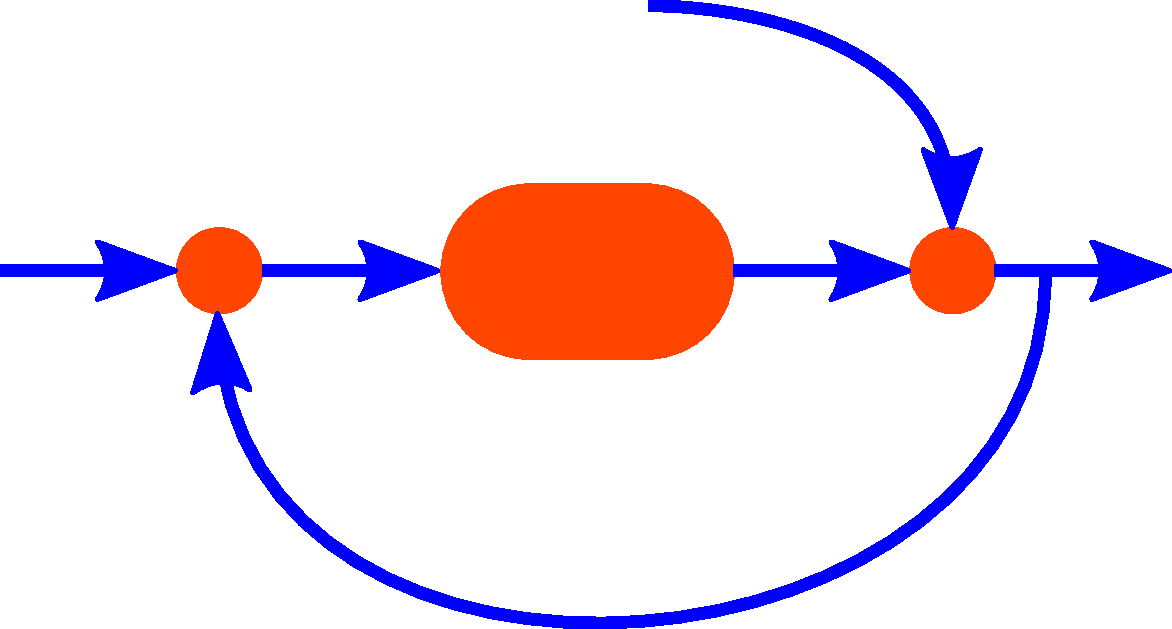
\includegraphics[scale=0.3]{./figuras/logos/logo_ltitool.png}


{\large \textit{\\LTI Control System Toolbox}}\\[4\baselineskip] % Tagline or further description
			{\large \textsc{ Eduardo J. Adam }} % Author name
			

\vspace{0.5\textheight} % Whitespace between the title block and the publisher
			{\noindent \textsc{A\~{n}o:} \Year }\\[\baselineskip] % Publisher and logo
	}$%
\lthtmlinlinemathZ
\lthtmlcheckvsize\clearpage}

\endgroup
\stepcounter{chapter}
\stepcounter{chapter}
\stepcounter{section}
\stepcounter{section}
\stepcounter{chapter}
{\newpage\clearpage
\lthtmldisplayA{displaymath258}%
\begin{displaymath}
	G(s)=\frac{b_m s^m \dots b_1 s + b_0}{s^n+a_1s^{n-1}+\dot a_{n-1}s^1 + a_n}
\end{displaymath}%
\lthtmldisplayZ
\lthtmlcheckvsize\clearpage}

{\newpage\clearpage
\lthtmldisplayA{displaymath264}%
\begin{displaymath}
	y(t)= \mathscr{L}^{-1} \left[ \frac{b_m s^m \dots b_1 s + b_0}{s^n+a_1s^{n-1}+\dot a_{n-1}s^1 + a_n} U(s)\right]
\end{displaymath}%
\lthtmldisplayZ
\lthtmlcheckvsize\clearpage}

\stepcounter{section}
{\newpage\clearpage
\lthtmlinlinemathA{tex2html_wrap_inline500}%
$\delta(t)$%
\lthtmlinlinemathZ
\lthtmlcheckvsize\clearpage}

{\newpage\clearpage
\lthtmlinlinemathA{tex2html_wrap_inline502}%
$u(t) = \delta(t)$%
\lthtmlinlinemathZ
\lthtmlcheckvsize\clearpage}

{\newpage\clearpage
\lthtmlinlinemathA{tex2html_wrap_inline504}%
$U(s) = \mathscr{L}[u(t)] = \mathscr{L}[\delta(t)] = 1$%
\lthtmlinlinemathZ
\lthtmlcheckvsize\clearpage}

{\newpage\clearpage
\lthtmldisplayA{displaymath281}%
\begin{displaymath} 
y(t) = \mathscr{L}^{-1}[G(s)] ~~\mbox{.}
\end{displaymath}%
\lthtmldisplayZ
\lthtmlcheckvsize\clearpage}

{\newpage\clearpage
\lthtmldisplayA{displaymath291}%
\begin{displaymath}
		G(s)=\frac{(s+1)}{s^2+ 0.5 s +1}
	\end{displaymath}%
\lthtmldisplayZ
\lthtmlcheckvsize\clearpage}

{\newpage\clearpage
\lthtmlfigureA{remark308}%
\begin{remark}
			\begin{remarca}
				The initial value ($t = 0^+$) of the impulse response of the self-regulating linear system itself with \textit{n} > \textit{m} is a finite magnitude.
			\end{remarca}
\par
\begin{demo}
				See Adam's textbook \cite{Adam2018}, among others.
			\end{demo}
		\end{remark}%
\lthtmlfigureZ
\lthtmlcheckvsize\clearpage}

{\newpage\clearpage
\lthtmldisplayA{eqnarraystar321}%
\begin{eqnarray*}
			y(0^{+}) &=& \lim _{s \to \infty } sG(s)U(s)\\
			&=& \lim _{s \to \infty } s \frac{(s+1)}{\left ( s^2 + 0.5 s + 1 \right ) } 1\\
			&=& 0  ~~\mbox{.}
		\end{eqnarray*}%
\lthtmldisplayZ
\lthtmlcheckvsize\clearpage}

{\newpage\clearpage
\lthtmlfigureA{remark330}%
\begin{remark}
			\begin{remarca}
				The final value ($t \to \infty$) of the impulse response of a self-regulating linear system itself with $n \ge m$\  is zero.
			\end{remarca}
\par
\begin{demo}
				See Adam's textbook \cite{Adam2018}, among others.
			\end{demo}
		\end{remark}%
\lthtmlfigureZ
\lthtmlcheckvsize\clearpage}

{\newpage\clearpage
\lthtmldisplayA{equationstar338}%
\begin{equation*} 
			y(\infty)= \lim _{s \to 0} s Y(s) = \lim _{s \to 0} s G(s)U(s) = \lim _{s \to 0} s \frac{(s+1)}{s^2+0.5 s+1}1=0
			~~\mbox{.}
		\end{equation*}%
\lthtmldisplayZ
\lthtmlcheckvsize\clearpage}

\stepcounter{section}
{\newpage\clearpage
\lthtmldisplayA{displaymath370}%
\begin{displaymath} 
y(t) =  \mathscr{L}^{^-1} \left[G(s) \frac{k}{s}  \right]   ~~\mbox{.}
\end{displaymath}%
\lthtmldisplayZ
\lthtmlcheckvsize\clearpage}

{\newpage\clearpage
\lthtmlfigureA{remark391}%
\begin{remark}
			\begin{remarca}
				The initial value of the step response of the self-regulating linear system itself is zero if \textit{n} > \textit{m} and nonzero if \textit{n} = \textit{m}.
			\end{remarca}
\par
\begin{demo}
				See Adam's textbook \cite{Adam2018}, among others.
			\end{demo}
		\end{remark}%
\lthtmlfigureZ
\lthtmlcheckvsize\clearpage}

{\newpage\clearpage
\lthtmldisplayA{equationstar404}%
\begin{equation*} 
			y(0^+)= \lim _{s \to 0} s Y(s) = \lim _{s \to 0} s \ G(s)U(s) =  \lim _{s \to \infty} \cancel{s} \frac{(s+1)}{s^2+0.5s+1} \frac{k}{\cancel{s}} = 0 ~~\mbox{.}
		\end{equation*}%
\lthtmldisplayZ
\lthtmlcheckvsize\clearpage}

{\newpage\clearpage
\lthtmlfigureA{remark415}%
\begin{remark}
			\begin{remarca}
				The final value of the step response of the self-regulating linear system itself is equal to \textit{kK}.
			\end{remarca}
\par
\begin{demo}
				See Adam's textbook \cite{Adam2018}, among others.
			\end{demo}
		\end{remark}%
\lthtmlfigureZ
\lthtmlcheckvsize\clearpage}

{\newpage\clearpage
\lthtmldisplayA{equationstar429}%
\begin{equation*} 
			y(\infty)= \lim _{s \to 0} s Y(s) = \lim _{s \to 0} s \ G(s)U(s) = \lim _{s \to 0} \cancel{s} \frac{(s+1)}{s^2+0.5s+1} \frac{k}{\cancel{s}} =  k
		\end{equation*}%
\lthtmldisplayZ
\lthtmlcheckvsize\clearpage}

\stepcounter{section}
{\newpage\clearpage
\lthtmldisplayA{displaymath463}%
\begin{displaymath}
	G(s)=\frac{s+1}{s^2+0.5s+1}
\end{displaymath}%
\lthtmldisplayZ
\lthtmlcheckvsize\clearpage}

\stepcounter{section}
\stepcounter{chapter}
{\newpage\clearpage
\lthtmlinlinemathA{tex2html_wrap_inline920}%
$G_t(s)=G_m(s)$%
\lthtmlinlinemathZ
\lthtmlcheckvsize\clearpage}

{\newpage\clearpage
\lthtmlinlinemathA{tex2html_wrap_inline922}%
$G(s)=G_p(s)G_v(s)G_m(s)$%
\lthtmlinlinemathZ
\lthtmlcheckvsize\clearpage}

{\newpage\clearpage
\lthtmlfigureA{theorem703}%
\begin{theorem}[Routh-Hurwitz stability Criterion] 

	The necessary and sufficient condition of stability is that all the terms in the first column of the Routh array have the same sign.
\end{theorem}%
\lthtmlfigureZ
\lthtmlcheckvsize\clearpage}

{\newpage\clearpage
\lthtmlinlinemathA{tex2html_wrap_inline924}%
$K_r$%
\lthtmlinlinemathZ
\lthtmlcheckvsize\clearpage}

{\newpage\clearpage
\lthtmlinlinemathA{tex2html_wrap_inline926}%
$T_I=5$%
\lthtmlinlinemathZ
\lthtmlcheckvsize\clearpage}

{\newpage\clearpage
\lthtmldisplayA{displaymath720}%
\begin{displaymath}
	G(s)H(s)=\frac{K_r\cancel{(5s+1)}}{5s}\frac{2}{\cancel{(5s+1)}(s^2+s+1)}=\frac{K^*}{s(s^2+s+1)}
\end{displaymath}%
\lthtmldisplayZ
\lthtmlcheckvsize\clearpage}

{\newpage\clearpage
\lthtmlinlinemathA{tex2html_wrap_inline928}%
$K^*=2K_r/5$%
\lthtmlinlinemathZ
\lthtmlcheckvsize\clearpage}

{\newpage\clearpage
\lthtmldisplayA{displaymath730}%
\begin{displaymath}
	\frac{Y(s)}{R(s)}=G_{lc}(s)=\frac{G(s)H(s)}{1+G(s)H(s)}=\frac{K^*}{s^3+s^2+s+K^*}.
\end{displaymath}%
\lthtmldisplayZ
\lthtmlcheckvsize\clearpage}

{\newpage\clearpage
\lthtmlinlinemathA{tex2html_wrap_inline930}%
$D(s)=s^3+s^2+s+K^*$%
\lthtmlinlinemathZ
\lthtmlcheckvsize\clearpage}

{\newpage\clearpage
\lthtmldisplayA{equationstar740}%
\begin{equation*}
	\begin{array} {c|}
		s^3 \\s^2 \\s^1 \\s^0
	\end{array}
	\begin{array} {cc}
		1  & 1 \\
		1  & K^* \\
		1-K^*  & 0  \\
		K^*  & 0 \\
	\end{array}
\end{equation*}%
\lthtmldisplayZ
\lthtmlcheckvsize\clearpage}

{\newpage\clearpage
\lthtmldisplayA{equationstar754}%
\begin{equation*} 
	y(0^+)= \lim _{s \to \infty} s Y(s) = \lim _{s \to \infty} s \ G_{lc}(s)R(s) =  \lim _{s \to \infty} \cancel{s} \frac{K^*}{s^3+s^2+s+K^*} \frac{k}{\cancel{s}} = 0 ~~\mbox{.}
\end{equation*}%
\lthtmldisplayZ
\lthtmlcheckvsize\clearpage}

{\newpage\clearpage
\lthtmldisplayA{equationstar766}%
\begin{equation*} 
	y(\infty)= \lim _{s \to 0} s Y(s) = \lim _{s \to 0} s \ G_{lc}(s)R(s) = \lim _{s \to 0} \cancel{s} \frac{K^*}{s^3+s^2+s+K^*} \frac{k}{\cancel{s}} =  k
\end{equation*}%
\lthtmldisplayZ
\lthtmlcheckvsize\clearpage}

{\newpage\clearpage
\lthtmlinlinemathA{tex2html_wrap_inline932}%
$D(s)=s^3+s^2+s+0.5$%
\lthtmlinlinemathZ
\lthtmlcheckvsize\clearpage}

{\newpage\clearpage
\lthtmlinlinemathA{tex2html_wrap_inline934}%
$s_1= -0.64780$%
\lthtmlinlinemathZ
\lthtmlcheckvsize\clearpage}

{\newpage\clearpage
\lthtmlinlinemathA{tex2html_wrap_inline936}%
$s_{2-3}=-0.17610 \pm j 0.86072$%
\lthtmlinlinemathZ
\lthtmlcheckvsize\clearpage}

\stepcounter{section}
\stepcounter{subsection}
{\newpage\clearpage
\lthtmlinlinemathA{tex2html_wrap_inline938}%
$K^*_u$%
\lthtmlinlinemathZ
\lthtmlcheckvsize\clearpage}

{\newpage\clearpage
\lthtmlinlinemathA{tex2html_wrap_inline940}%
$\omega_{-180}$%
\lthtmlinlinemathZ
\lthtmlcheckvsize\clearpage}

{\newpage\clearpage
\lthtmlinlinemathA{tex2html_wrap_inline942}%
$\omega_{cg}$%
\lthtmlinlinemathZ
\lthtmlcheckvsize\clearpage}

{\newpage\clearpage
\lthtmlinlinemathA{tex2html_wrap_inline944}%
$K^* = 0.5$%
\lthtmlinlinemathZ
\lthtmlcheckvsize\clearpage}

{\newpage\clearpage
\lthtmlinlinemathA{tex2html_wrap_inline950}%
$K^*$%
\lthtmlinlinemathZ
\lthtmlcheckvsize\clearpage}

\stepcounter{subsection}
\stepcounter{section}
\stepcounter{chapter}
\stepcounter{section}
\stepcounter{section}
\stepcounter{section}
\stepcounter{subsection}
\stepcounter{subsection}
\stepcounter{section}
\stepcounter{chapter}
\stepcounter{section}
\stepcounter{section}
\stepcounter{subsection}

\renewcommand{\headrulewidth}{0pt}
\appendix

\end{document}
